\documentclass[]{report}
\usepackage{listings,graphicx}
\usepackage{float}
\graphicspath{{resources/}}

% Title Page
\title{WhisPeerer \\A WebRTC communications application}
\author{Dominic Rathbone \\ Student Number: 12843140 \\ Source Code \& Documentation: \\ https://github.com/domr115/CI360-Mobile-App-Dev}


\begin{document}
\maketitle

\tableofcontents

\chapter{Introduction}
The aim of this project was to provide an application enabling users to communicate using peer-to-peer technology. The motivation behind this was the increasing concern of security many consumers face in the modern age due to third parties, whether it be a corporation such as Facebook or an authority such as the UK Government, storing and analysing their data. By using a technology called WebRTC, it is possible for two users to form a direct peer to peer connection over the internet.  Although a server is used for the initial signalling and negotiation process between the peers, the communication data sent over this communications channel is never disclosed to an external server. On top of this, the application aimed to provide a sense of anonymity and impermanence by only providing users with a temporary, random unique identifier for a user-name and only storing data within the lifespan of the application.

	\chapter{Development}
		\section{Node.js Signalling Server}
			\subsection{API}
			In order to set up a space in which two users can exchange the meta-data needed for the negotiation of a peer connection, an API was created on the server using Express.js, a popular web application framework for Node.js. This consists of two endpoints, one endpoint to create a new user and one endpoint to check if the user exists. The former returns a unique, random session identifier to the application and the latter simply returns a status code of 200 or 404 dependent on whether the user exists or not. s. This API was designed using the Representation State Transfer (REST) architectural style in order to provide a uniform and consistent API to it's consumers. REST achieves this by modelling the endpoints in an API around the resources they represent with HTTP verbs representing the operations that are achievable on this resource. For example, in order to create a user on the server, the consumer send a POST request to a "/user" endpoint and in order to check if a user exists, the consumer sends a GET request to "/users/[userId]". This architectural style also makes the API more extensible as it is easy to design new endpoints.
			
			\subsection{WebSockets}
			To provide a bi-direction communications channels for the two application instances to negotiate the peer connection over, a WebSockets implementation called Socket.io was used. Socket.io models communication using the concepts of name spaces and rooms where a name space is represented by the endpoint a socket connects to and rooms are channels within this that users can join and leave. In this case, each user is represented by their own namespace "/user/[userId]". When another user wants to communicate with a user, they join their namespace, becoming a "guest". In turn, this puts it into a "busy" state preventing other users from joining. From this namespace, the two users can exchange messages and once they are done and the guest disconnects, taking it out of the "busy" state. By modelling the user's communications channels like this, the guest user can still receive incoming chat offers from other users whilst busy with another user, similar to how a mobile phone can still receive calls whilst in a call with another. 
			
		\section{Android Application}
			
			\subsection{Architecture}
			As the majority of the data processing is handled by the libraries, the application's responsibilities mainly lied in the triggering of and reaction to incoming messages from another instance of the application, whether it be through the signalling server or directly via the peer-to-peer connection. Due to this, the architecture of the application can be represented by an "Event-Driven Architecture" pattern. This is where the flow of control in an application is dictated by the emission of and reaction to "events" where an event is a change in the state of the application. The overall architecture of the system the application belongs to can be broken down into 3 layers, the presentation layer, the communications layer and the server with the communications layer being the basis on which the user interface retrieves information from another instance of the application.
			
			\begin{figure}[H]
			\caption{Application Architecture}
			\includegraphics[scale=0.35]{Architecture.png}
			\end{figure}	
					
			\subsection{Design Patterns}
			To create the event-driven architecture, the application utilises the Observer pattern to trigger changes in the flow of the application by asynchronously updating activities (and thus the user interface) when certain events are received. The observer pattern is a design pattern in which two types of objects are implemented, "Observers" and "Observables". Each Observer overrides a set of methods that are called when an event on the "Observable" object happens and then adds itself to a list of observers on the observable objects. When an event occurs on this observable object, it goes through the list of observers, calling the corresponding event method. In this case, the observer pattern was chosen as activities such as the one that represents an incoming call activity needed to be instantiated spontaneously throughout the application. By using the observer pattern, the current activity could assign itself as the observer for the signaller (implementing the observable interface), updating the activity when the signaller received an "offer" for an incoming call.
			
			As the majority of the "events" within the application took the form of JSON messages transmitted and received from another application instance over the WebSockets connection with the server, the Java client library for Socket.io also used the Observer pattern. However, as the library was the one supplying the observables. The application only needed to supply the observers by passing through anonymous classes implementing the library-specific "Listener" interface when setting up these events. This interface requires the object to implement methods with the code that is to be called when the event is received (see Appendix A for an example). Further to this, the application also interacts with the server through a HTTP API, prior to establishing a signalling session with WebSockets. To react to  a success or failure of the requests sent to the API, a handler is passed through that methods representing the code that should be executed in either case.
			
			The application also uses the factory pattern in order to produce media streams to send to the other user through the peer connection. The factory pattern obfuscates the process of creating these media streams away from the object that called them, meaning it only has to supply the options for the object they want the factory to create (in this case, a parameter is passed through specifying whether a video stream should be added).
			
		\section{Communications Layer}
		To communicate with the server and other application instances, the application makes use of various libraries to implement a number of communications protocols. 
		
			\subsection{Android Asynchronous HTTP Client}
			The first of these is the Android Asynchronous HTTP Client library. This library was used as it made it easy to send asynchronous HTTP requests to the node server. A static class was created that mapped each endpoint of the HTTP API to a method which the activities could then call, passing parameters such as a username and a handler with the code that they wanted executed when the result was returned. The library then executed this request by adding it to a queue from which a pool of threads picks from, passing through the handler with it.
	
			\subsection{WebRTC/LibJingle}
			The application uses WebRTC to form a peer-to-peer connection using a offer-answer negotiation process. The offer and answer are formatted using the "Session Description Protocol" (SDP) and contain the parameters that represent what each peer wants from the connection such as media constraints (See Appendix B for an example). The initiating application creates a peer connection object and then a "offer" SDP which is sent over WebSockets to the server, forwarding it on to the destination application. This application, listening for socket events, receives the SDP and sets it as the remote description. After doing so, they generate an "answer" SDP and sends it back to the offerer. Once they both have the SDPs, the library can extract the parameters from them to connect the two peer connection objects. From this, the application creates a media stream that can contain the live streaming video from the application and the audio from the microphone and adds it to this peer connection. This media stream is sent over a protocol called SRTP. SRTP is an extension to the real-time protocol (RTP) that provides more security features such as authentication and encryption. RTP is a protocol that usually sits on top of the UDP transport protocol and is used for media streaming over a network and therefore is primarily used in telephony and video conferencing applications. Although it uses UDP and doesn't provide any mechanisms for reliability or quality of the data in the stream, it is supported by another protocol called Real-Time Control Protocol (RTCP) which monitors the transmission of data in order to provide statistics on the quality of service provided by RTP. This way, the statistics can be sent to participants of the stream and measures can be taken to detect and fix faults in this transmission. 
						
			
			\subsection{Socket.io Java Client}
			To provide a method of bi-directional communication that is necessary for the negotiation process used by WebRTC, the server uses Socket.io. To support this on the client application, it uses a un-official library that is based on the official socket.io java engine library to provide an interface into it. In turn, this library uses HTTP to upgrade the connection between the socket.io server and the client to use the WebSockets (WSS) protocol, from which it can send messages to or receive messages from the server. If this upgrade is not possible, it falls back on long polling the server using HTTP requests. WebSockets was chosen as the protocol for bi-directional communication as even though the application is not browser-based at the moment, if the platform was expanded to include a browser-based web application, it would mean that the android application would be able to communicate with it. If node.js was to use plain TCP sockets instead, this would not be possible.
		
		\section{Presentation Layer}
		Using the observer pattern described earlier, each activity making up the presentation layer was able to and subscribe to parts of the communication layer for updates from the server and other application instance and send updates through it. 
		
		\subsection{Home Activity}
			\begin{figure}[H]
				\caption{Home Activity}
				\centering
				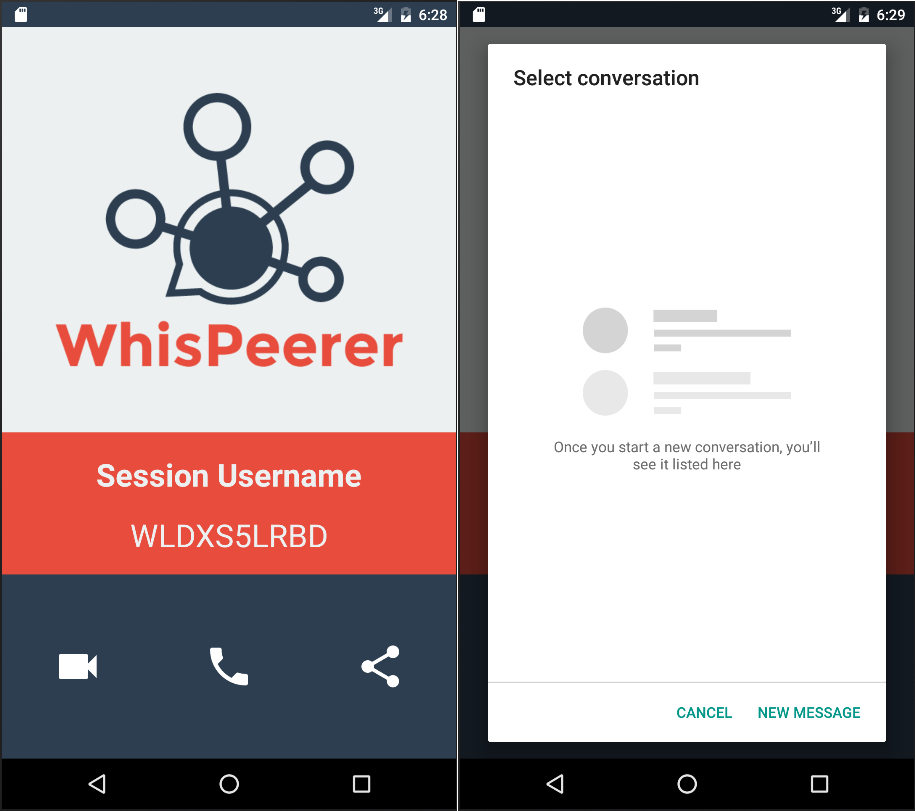
\includegraphics[scale=0.35]{HomeActivity.png}
			\end{figure}		
		The home activity is the entry point into the application. Due to this, this is where the application is setup to be able to receive messages from another instance. To do this, a HTTP request is sent to the server, creating a name space in which other users can connect to with WebSockets. The response to this request returns a unique identifier for the user's session. With this response, the application connects to the name space by creating a new Signaller instance and sets itself as the observer to this instance so it can listen for incoming events. From this activity, the user can either initiate the process to start a video or voice chat as well as share their session username via an intent.
		\subsection{Start Chat Activity}
			\begin{figure}[H]
				\caption{Start Chat Activity}
				\centering
				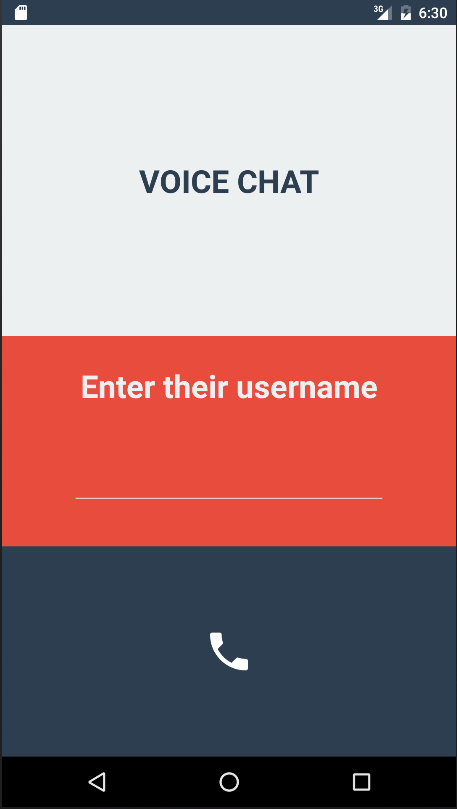
\includegraphics[scale=0.35]{StartChatActivity.png}
			\end{figure}
		\subsection{Chat Activity}
			\begin{figure}[H]
				\caption{Chat Activity}
				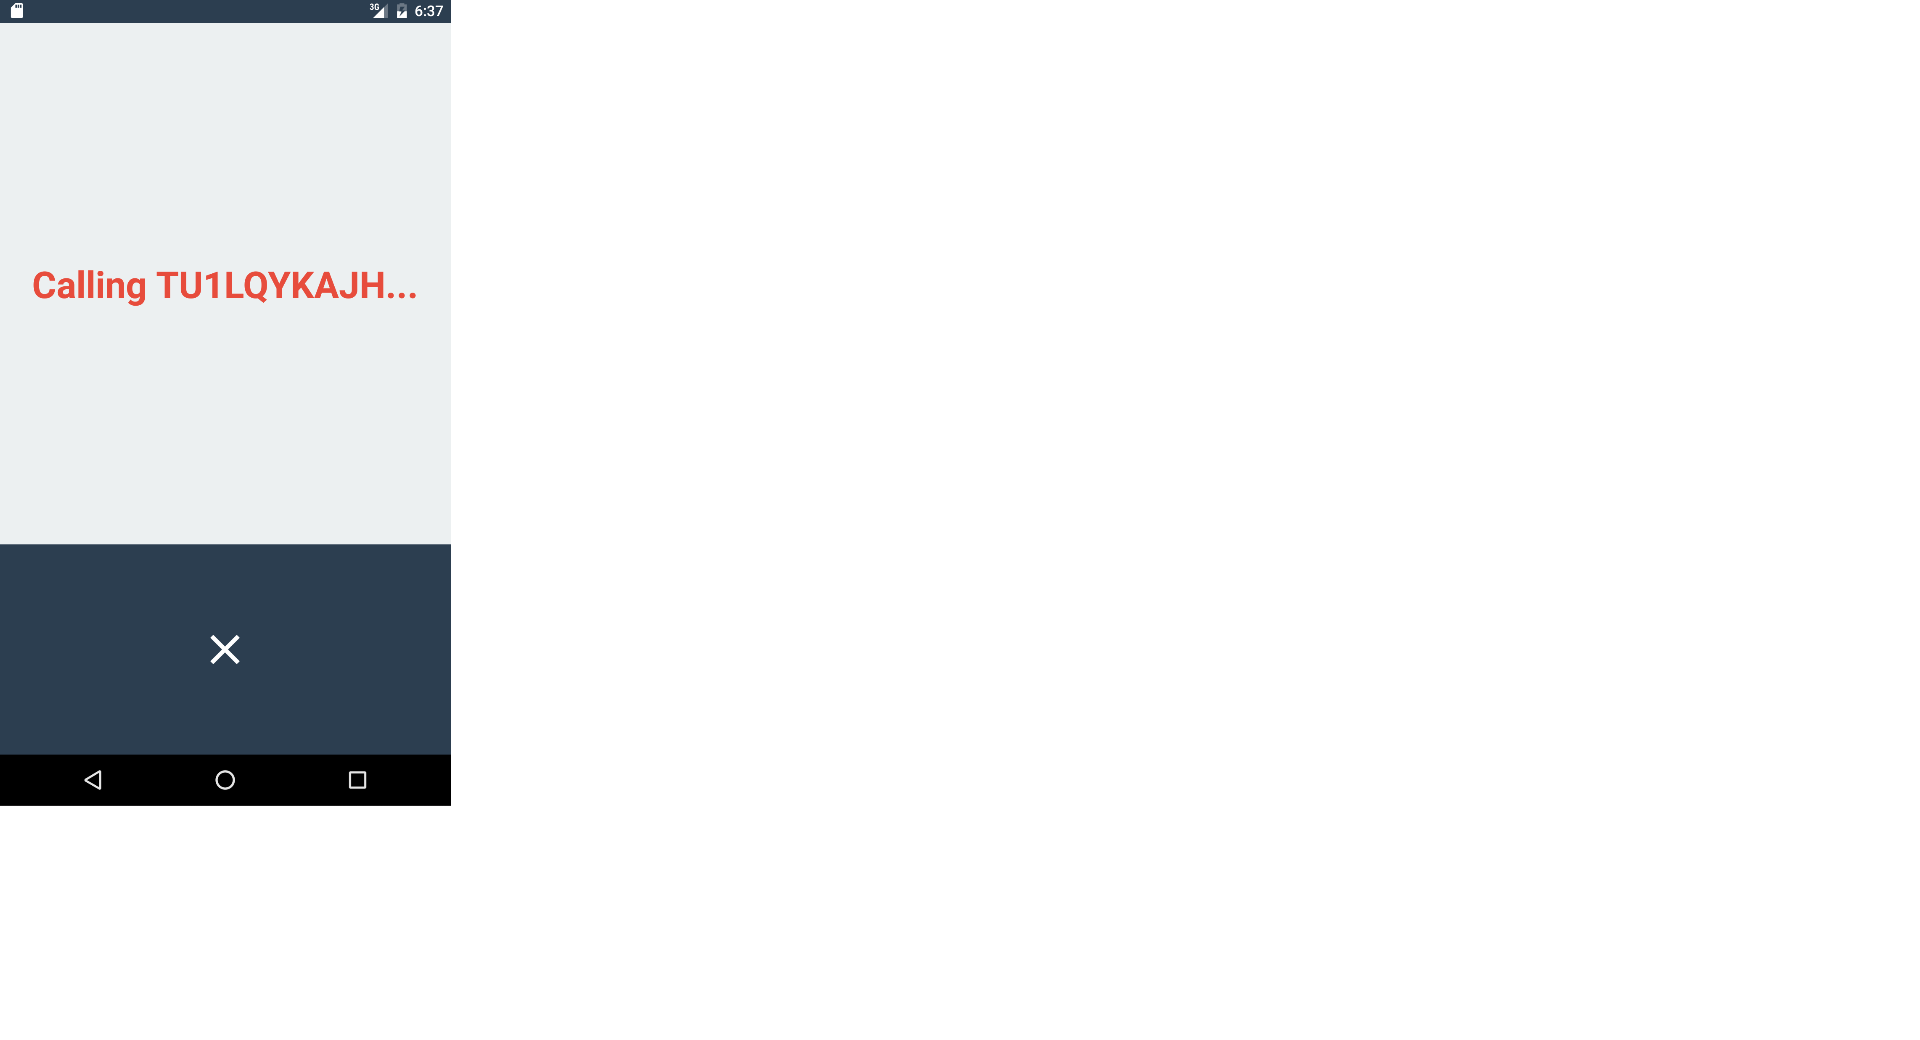
\includegraphics[scale=0.35]{ChatActivity.png}
			\end{figure}
		\subsection{Chat Display Activity}
			\begin{figure}[H]
				\caption{Chat Activity}
				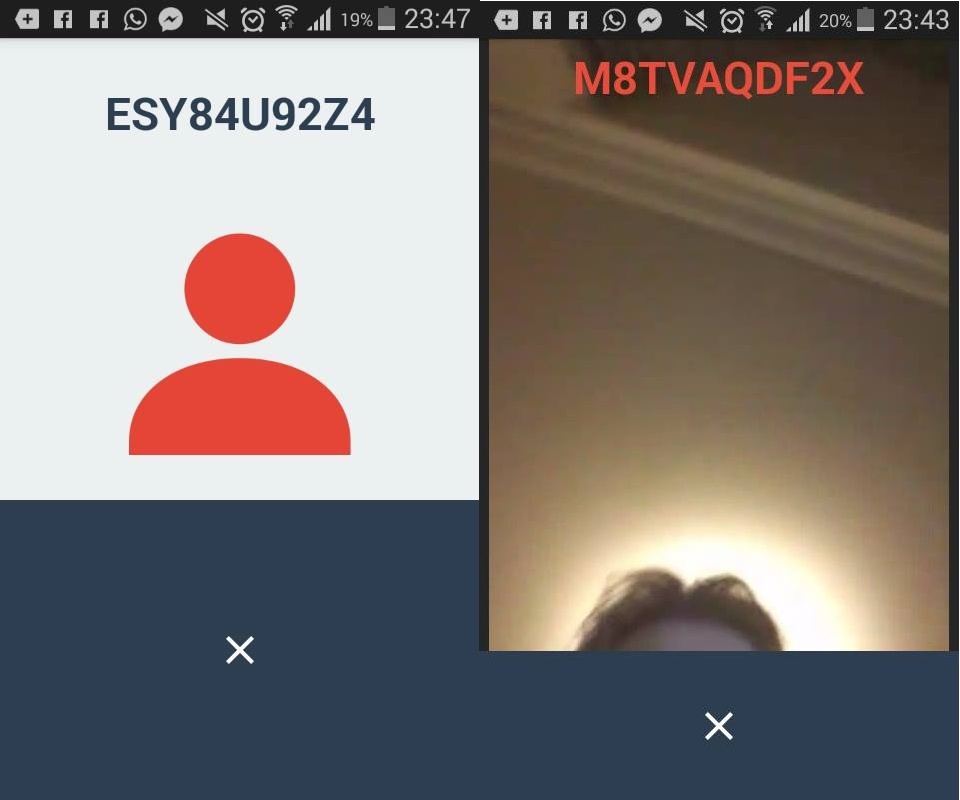
\includegraphics[scale=0.35]{ChatDisplayActivity.png}
			\end{figure}
		
		\section{Utilities}
			
		\section{Other Libraries}
		Camera
		Microphone
		Vibrator
		Share
		
	\section{External Technologies}
		\section{Git}
		\section{Android Studio}
		\section{WebStorm}
		
	\chapter{Design}
		As the application used relative new technologies, the majority of the project was focused on developing around these to ensure they worked. Due to this, the design aspect of the project was considered a lower priority.
		\section{Logo}
		\section{Color Scheme}
		\section{Layout}

	\chapter{Testing}
		\section{Automated Testing}
			\subsection{Unit Tests}
		\section{Manual Testing}
	
	\chapter{Reflection \& Review}
		\section{Background Research}
		\section{Methodology}
		\section{Project Estimation}
		\section{Development Process}
			\subsection{Debugging}
		\section{Application Improvements}
			\subsection{Web to Native Application Communication}
		\section{Conclusion}
	
	\appendix
	\chapter{}
		\chapter{}
		\begin{figure}[h!]
			\caption{Observer Pattern}
			\begin{lstlisting}[language=Java,frame=single,breaklines=true]
			
			\end{lstlisting}
		\end{figure}
	\begin{figure}[h!]
		\caption{Socket Event Listener}
		\begin{lstlisting}[language=Java,frame=single,breaklines=true]
socket.on("offer", new Emitter.Listener() {
	@Override
	public void call(Object... args) {
		
	}
})
		\end{lstlisting}
	\end{figure}
	
\begin{figure}[h!]
	\caption{Socket Event Listener}
	\begin{lstlisting}[tabsize=1,frame=single, basicstyle=\ttfamily\footnotesize, breaklines=true]
	//Global Parameters
	v=0
	o=- 8673508164875365281 2 IN IP4 127.0.0.1
	s=-
	t=0 0
	a=group:BUNDLE audio video data
	a=msid-semantic: WMS
	//Audio Parameters
	m=audio 55386 UDP/TLS/RTP/SAVPF 111 103 104 9 0 8 106 105 13 126
	c=IN IP4 81.132.56.236
	a=rtcp:55388 IN IP4 81.132.56.236
	//ICE Candidates
	a=candidate:186199869 1 udp 2113937151 192.168.1.101 55386 typ host generation 0
	a=candidate:186199869 2 udp 2113937150 192.168.1.101 55388 typ host generation 0
	a=candidate:842163049 1 udp 1677729535 81.132.56.236 55386 typ srflx raddr 192.168.1.101 rport 55386 generation 0
	a=candidate:842163049 2 udp 1677729534 81.132.56.236 55388 typ srflx raddr 192.168.1.101 rport 55388 generation 0
	//ICE Parameters
	a=ice-ufrag:0wQWmUu1vNtLfQb+
	a=ice-pwd:CypcDjpI4jVplwdXcYFUDBAx
	//DTLS Parameters
	a=fingerprint:sha-256 46:11:61:1B:E1:D4:75:30:19:1A:50:11:73:F3:5C:3F:DA:D0:2C:D3:6F:E3:CE:EB:1E:13:94:12:00:71:51:60
	a=setup:actpass
	a=mid:audio
	a=extmap:1 urn:ietf:params:rtp-hdrext:ssrc-audio-level
	a=extmap:3 http://www.webrtc.org/experiments/rtp-hdrext/abs-send-time
	a=recvonly
	a=rtcp-mux
	//Codec Parameters
	a=rtpmap:111 opus/48000/2
	a=fmtp:111 minptime=10; useinbandfec=1
	a=rtpmap:103 ISAC/16000
	a=rtpmap:104 ISAC/32000
	a=rtpmap:9 G722/8000
	a=rtpmap:0 PCMU/8000
	a=rtpmap:8 PCMA/8000
	a=rtpmap:106 CN/32000
	a=rtpmap:105 CN/16000
	a=rtpmap:13 CN/8000
	a=rtpmap:126 telephone-event/8000
	a=maxptime:60
	//Video Parameters
	m=video 55392 UDP/TLS/RTP/SAVPF 100 101 116 117 96
	c=IN IP4 81.132.56.236
	a=rtcp:55394 IN IP4 81.132.56.236
	//ICE Candidates
	a=candidate:186199869 1 udp 2113937151 192.168.1.101 55392 typ host generation 0
	a=candidate:186199869 2 udp 2113937150 192.168.1.101 55394 typ host generation 0
	a=candidate:842163049 2 udp 1677729534 81.132.56.236 55394 typ srflx raddr 192.168.1.101 rport 55394 generation 0
	a=candidate:842163049 1 udp 1677729535 81.132.56.236 55392 typ srflx raddr 192.168.1.101 rport 55392 generation 0
	//ICE Parameters
	a=ice-ufrag:0wQWmUu1vNtLfQb+
	a=ice-pwd:CypcDjpI4jVplwdXcYFUDBAx
	//DTLS Parameters
	a=fingerprint:sha-256 46:11:61:1B:E1:D4:75:30:19:1A:50:11:73:F3:5C:3F:DA:D0:2C:D3:6F:E3:CE:EB:1E:13:94:12:00:71:51:60
	a=setup:actpass
	a=mid:video
	a=extmap:2 urn:ietf:params:rtp-hdrext:toffset
	a=extmap:3 http://www.webrtc.org/experiments/rtp-hdrext/abs-send-time
	a=extmap:4 urn:3gpp:video-orientation
	a=recvonly
	a=rtcp-mux
	//Codec Parameters
	a=rtpmap:100 VP8/90000
	a=rtcp-fb:100 ccm fir
	a=rtcp-fb:100 nack
	a=rtcp-fb:100 nack pli
	a=rtcp-fb:100 goog-remb
	a=rtcp-fb:100 transport-cc
	a=rtpmap:101 VP9/90000
	a=rtcp-fb:101 ccm fir
	a=rtcp-fb:101 nack
	a=rtcp-fb:101 nack pli
	a=rtcp-fb:101 goog-remb
	a=rtcp-fb:101 transport-cc
	a=rtpmap:116 red/90000
	a=rtpmap:117 ulpfec/90000
	a=rtpmap:96 rtx/90000
	a=fmtp:96 apt=100
	m=application 55390 DTLS/SCTP 5000
	c=IN IP4 81.132.56.236
	//ICE Candidates
	a=candidate:186199869 1 udp 2113937151 192.168.1.101 55390 typ host generation 0
	a=candidate:842163049 1 udp 1677729535 81.132.56.236 55390 typ srflx raddr 192.168.1.101 rport 55390 generation 0
	//ICE Parameters
	a=ice-ufrag:0wQWmUu1vNtLfQb+
	a=ice-pwd:CypcDjpI4jVplwdXcYFUDBAx
	//DTLS Parameters
	a=fingerprint:sha-256 46:11:61:1B:E1:D4:75:30:19:1A:50:11:73:F3:5C:3F:DA:D0:2C:D3:6F:E3:CE:EB:1E:13:94:12:00:71:51:60
	a=setup:actpass
	a=mid:data
	a=sctpmap:5000 webrtc-datachannel 1024
	\end{lstlisting}	
\end{figure}
\end{document}          
